\documentclass[10pt,a4paper,twocolumn]{article}
\usepackage[T1]{fontenc}
\usepackage[utf8]{inputenc}
\usepackage{newtxtext,newtxmath}
\usepackage[top=18mm,bottom=19mm,left=16mm,right=16mm,columnsep=6mm]{geometry}
\usepackage{graphicx,booktabs,tabularx,array,amsmath,microtype,caption,titlesec,dblfloatfix}
\usepackage{tikz}
\usepackage[hidelinks,breaklinks]{hyperref}
\usepackage{url}
\urlstyle{same}
\graphicspath{{figures/}}
\DeclareCaptionFont{cirpcaption}{\fontsize{8.5}{10}\selectfont}
\captionsetup{font=cirpcaption,labelfont=normalfont,labelsep=period,skip=5pt}
\titleformat{\section}{\normalsize\bfseries}{\thesection.}{.5em}{}
\titleformat{\subsection}{\normalsize\itshape}{\thesubsection.}{.5em}{}
\titlespacing*{\section}{0pt}{10pt}{5pt}
\titlespacing*{\subsection}{0pt}{8pt}{4pt}
\setlength{\parindent}{1em}
\setlength{\parskip}{0pt}
\setlength{\textfloatsep}{11pt plus 2pt minus 2pt}
\setlength{\dbltextfloatsep}{11pt plus 2pt minus 2pt}
\setcounter{topnumber}{3}
\setcounter{dbltopnumber}{3}
\renewcommand{\topfraction}{.92}
\renewcommand{\dbltopfraction}{.92}
\renewcommand{\textfraction}{.06}
\renewcommand{\floatpagefraction}{.8}
\newcommand{\ndcg}{\mathrm{nDCG}}
\newcommand{\Full}{\textit{Full}}
\newcommand{\Proposed}{\textit{KG--LLM}}

\begin{document}
\fontsize{9.5}{11.3}\selectfont
\twocolumn[{
\begin{minipage}{\textwidth}
{\LARGE\bfseries\raggedright Knowledge-guided relational evidence\\for functional CAD retrieval\par}
\vspace{9pt}
\small
Functional CAD reuse requires evidence of role-specific interfaces. A knowledge graph (KG) specifies relational geometric requirements, visual language models assess candidate views, and deterministic coverage refines retrieval under measured size constraints. Evaluation uses 1,816 CADs and 264 queries across eleven roles with AI-derived relevance judgments. Three response collections per observer assess acquisition variability. KG-directed GPT-6 Luna achieves nDCG@5 of 0.8254 and 0.8125 for embeddings and descriptors. Differences from matched holistic role assessment are +0.0447 and +0.0210. Component ablation separates numerical eligibility, role priors and visual evidence; corrected tests remain inconclusive.

\par\vspace{6pt}
Computer aided design (CAD); Knowledge based system; Design reuse; Knowledge graph
\par\vspace{12pt}
\end{minipage}
}]

\section{Introduction}

CAD reuse depends on finding components that satisfy a design role as well as geometric requirements. A belt drive requires an appropriate contact profile; shaft transmission requires a drive interface; tension return requires attachments at the ends of a spring. Similar overall shape can coexist with different interface functions. Connecting computational representations to this engineering context is central to data-driven design \cite{liu2024datadriven}. Functional retrieval therefore requires an explicit connection between a requested role and evidence from the individual candidate.

Mechanical-part retrieval combines geometric, topological and feature information \cite{chu2006similarity}. Learned boundary representations, including UV-Net \cite{jayaraman2021uvnet} and boundary-representation transformers \cite{zou2025brt}, extend the information available for shape comparison. Network modelling also supplies structured representations of three-dimensional objects in manufacturing \cite{yang2020network}. Design knowledge management links layout and function \cite{koh2003design}, while knowledge representation preserves engineering context \cite{chandrasegaran2013knowledge}. In retrieval, ontology-based integration \cite{qin2016ontology}, semantic bipartite matching \cite{han2018semantics} and graph-based multi-criteria assembly retrieval \cite{lupinetti2018multicriteria} provide established ways to incorporate this context. Query objectives, descriptors and matching criteria remain central methodological choices \cite{lupinetti2019survey}.

Large language models (LLMs) extend semantic access to design information. LLM query planning coordinates vector, structural and attribute retrieval for CAD models \cite{lv2026cognitive}; graph-linked design documents support contextual retrieval \cite{theuner2025weaving}; and retrieval-augmented generation extracts schema-directed information from native CAD assemblies \cite{kurscheid2026extracting}. Vision-language models also recognize manufacturing features from CAD views \cite{khan2025leveraging}. Their broader engineering assessment identifies substantial variation across geometric tasks \cite{picard2025concept}. These capabilities motivate a specific internal role in retrieval: acquiring observations for the geometric relationships required by the requested function.

This paper presents a knowledge-guided visual-evidence framework for functional CAD retrieval. A typed knowledge graph (KG) specifies role-dependent geometric predicates and component bindings. An LLM observes these predicates in candidate views; deterministic coverage then augments geometric similarity, exemplar-category agreement and class-derived function support. Measured dimensions determine eligibility. The contributions are role-directed acquisition of instance-level relational evidence, its integration with a source-linked retrieval process, and a repeated-collection comparison with holistic visual assessment across eleven design-role families. The method addresses fine role distinctions that a broad category prior leaves unresolved.

\section{Knowledge-guided CAD retrieval}

\subsection{Evidence representation}

Figure~\ref{fig:framework} illustrates the framework. Part, Class, Function and Measurement records connect source geometry, model predictions, scoped engineering associations and dimensional evidence. Role--Predicate relations specify required features and their component bindings. Observation records contain a model-assessed state, cited views, a geometric description and source-image/model identity. Predicted-category support, visual observations and measured eligibility retain their respective provenance.

\begin{figure*}[t]
\centering
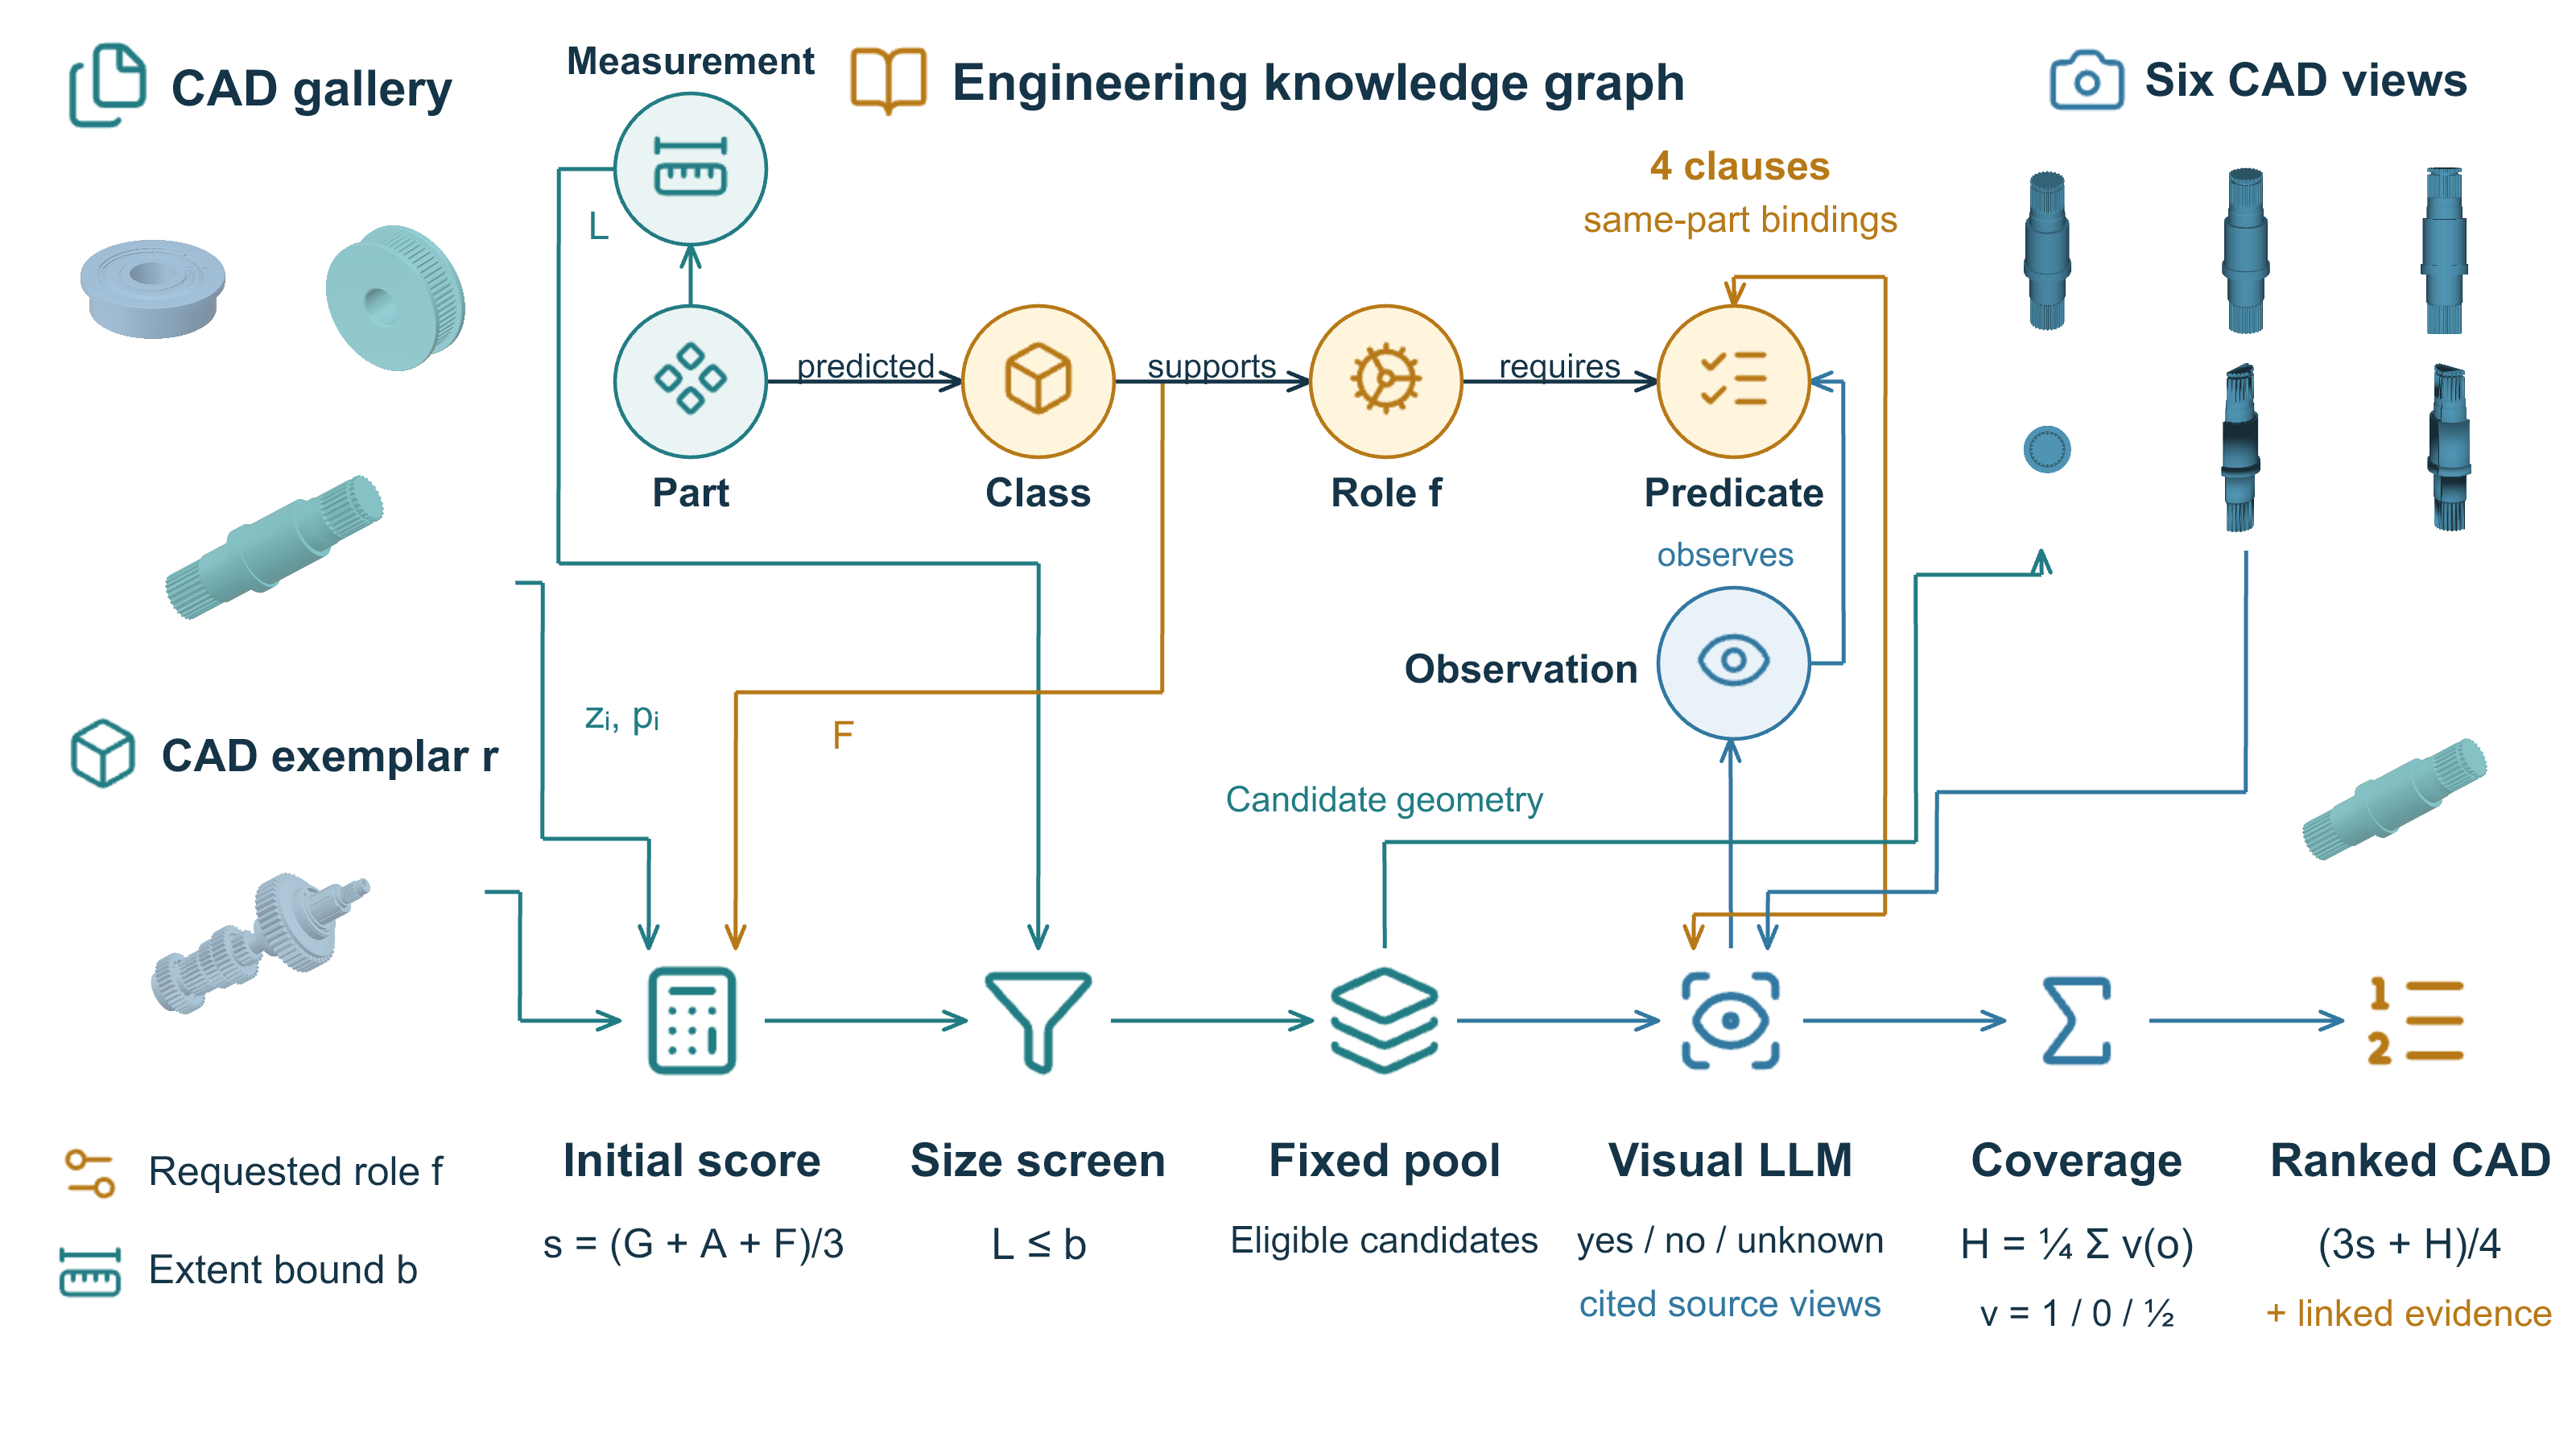
\includegraphics[width=\textwidth]{framework_redrawn.png}
\caption{Knowledge-guided CAD retrieval. Source geometry and predicted categories supply $G,A,F$, while measured extents determine size eligibility $C$. The KG binds the requested role to four geometric predicates and their component relationships. Candidate views and these clauses enter the visual LLM, which records states and cited views. Deterministic coverage $H$ refines the eligible pool by $(3s+H)/4$. CAD inserts show actual source geometries at independent display scales with illustrative ceramic materials. The view montage reproduces an archived input, including two display clips. OpenAI image generation assisted the layout concept; the final diagram uses editable graphics and source CAD renders.}
\label{fig:framework}
\end{figure*}

A query supplies a requested role $f$, a CAD exemplar $r$ and an optional largest-extent upper bound $b$. Class--function associations originate from manufacturer references covering bearings, couplings, belt drives, fasteners, brackets, flanges, gears, shafts and springs. Their scopes appear in Supplementary Section~S2; engineering sources accompany the role-association data. These associations provide category-level support; role predicates express visible requirements at the candidate level.

Geometry is represented by a 128-dimensional supervised local-surface embedding or a 13-dimensional descriptor. The descriptor contains dimension ratios, box fill and surface ratios, entity counts, and surface/edge-type fractions. Training medians impute missing components; training means and standard deviations define normalization. The embedding and ten-class prediction head use the same validation-selected checkpoint throughout. Supplementary Section~S1 provides the coordinates, architecture and model identities.

\subsection{Initial ranking and dimensional eligibility}

Let $\boldsymbol z_i$ denote candidate $i$ and $\boldsymbol p_i$ its predicted distribution over ten classes. Geometric similarity and exemplar-category agreement are
\begin{align}
G_i&=\tfrac12\{1+\cos(\boldsymbol z_i,\boldsymbol z_r)\},\label{eq:geometry}\\
A_i&=\boldsymbol p_i^{\mathsf T}\boldsymbol p_r.\label{eq:agreement}
\end{align}
For requested role $f$, class-derived function support is
\begin{equation}
F_i(f)=\sum_c p_i(c)\rho_{cf}\eta_{cf},\label{eq:function}
\end{equation}
where $\rho_{cf}$ and $\eta_{cf}$ denote relevance and inclusion weights. Each evaluated role has one admitted class association with both weights equal to one, so $F_i$ is the corresponding predicted class probability. Compression and tension return share the spring class and therefore the same prior. Source labels qualify the generic association rather than annotating an individual CAD.

The initial ranker, denoted Base \Full, uses equal component weights:
\begin{equation}
s_i=(G_i+A_i+F_i)/3.\label{eq:base}
\end{equation}
The physical screen $C$ admits a candidate when its verified largest stored-axis extent satisfies
\begin{equation}
L_i=\max_{a\in\{x,y,z\}}(x^{\max}_{ia}-x^{\min}_{ia})\leq b.\label{eq:extent}
\end{equation}
STEP-kernel processing supplies values, explicit units and validity status. Failed or unknown measurements are excluded from a bounded request. The criterion evaluates the file coordinate system; an unbounded query admits the common gallery. Exact score ties are resolved by part identity.

\subsection{KG-directed visual observation}

The requested role selects four geometric clauses and their required triples. Each clause binds its feature to the relevant body or interface. Tension return requires a helical coil, a terminal hook at one end, another hook at the other end, and their attachment to opposite ends of the same coil. Shaft transmission requires an elongated body, journal regions along it, a drive feature on that body and rotary shaft form. Thus a feature's presence and its placement contribute explicit evidence. Supplementary Table~S1 summarizes all forty-four clauses.

Each candidate is shown in six existing orthographic views: oblique, opposite, profile, axial and two uncapped visual clips. The 1500$\times$1000 input montage preserves CAD geometry and view arrangement, with descriptive titles removed. The instructions distinguish display cuts from actual through-passages. The model receives the requested predicates and triples with these views. Class labels, probabilities, ranks, relevance grades and exemplar identities remain outside this input.

The evaluated GPT-6 Luna and GPT-6.1 Sol observers return a structured observation for every clause: \textit{yes}, \textit{no} or \textit{unknown}, with supporting view names and a short geometric description. Visible evidence supports yes or no; occlusion, simplified representation and ambiguity receive unknown. Observations are stored once per role--CAD pair and reused across exemplars, size conditions and geometry representations. Collection uses low reasoning effort, a 2,000-token output cap and the same strict output schema throughout. Each observation records its source view and model provenance.

\subsection{Coverage and refined ranking}

For observed state $o_{ifk}$ of clause $k$, the evidence value and role coverage are
\begin{equation}
v(o)=\begin{cases}1,&o=\mathrm{yes},\\0,&o=\mathrm{no},\\1/2,&o=\mathrm{unknown},\end{cases}
\qquad H_i(f)=\frac14\sum_{k=1}^{4}v(o_{ifk}).\label{eq:coverage}
\end{equation}
Coverage is a soft ranking signal with retained observation states and provenance. Model observations enter this signal; verified measurements continue to determine dimensional eligibility.

For each query and representation, a refinement pool takes the union of the first ten eligible candidates from Base \Full, $G+F+C$ and $G+C$. The proposed method, denoted \Proposed, ranks this pool by
\begin{equation}
S_i^{\mathrm{KG\mbox{--}LLM}}=\frac{G_i+A_i+F_i+H_i(f)}4
=\frac{3s_i+H_i(f)}4.\label{eq:refined}
\end{equation}
The original components and the added signal therefore have equal weights. The reranked pool precedes the unchanged Base \Full{} tail, with part identity breaking ties. Each pool includes the original top five of these three branches. This bounded acquisition step adds instance-level visual evidence while retaining the same source gallery and numerical requirement. Supplementary Section~S2 specifies the complete observation contract and fallback policy.

\subsection{Repeated acquisition and role-only controls}

Each observation design is evaluated in three response collections: KG-directed
GPT-6 Luna, KG-directed GPT-6.1 Sol and holistic role-only GPT-6 Luna. The gallery,
images, requested requirements, output schema and scoring weights are fixed.
Collections assess variation in model observations under a common representation
checkpoint. The first KG collection for each model precedes the interleaved
repetitions; the API provides no sampling-seed control. A failed assessment
receives neutral support of one half, as specified before acquisition.

The role-only observer receives the requested role's purpose and the same six views,
without the four authored clauses, triples or component-binding instructions.
Generic guidance on uncertainty, display clips and the limits of visible geometry
is retained. It reports holistic visual support $J_i$ from
$\{0,\frac18,\ldots,1\}$, with cited views and a literal explanation. This matches
the range and increments of $H_i$. The same-model control substitutes $J_i$ for
$H_i$ in Eq.~\ref{eq:refined}, preserving the initial score, pool and dimensional
screen. A score-only LLM control ranks the same eligible pool by $J_i$ alone.
Its serving score omits $G,A,F$, while its candidate access remains conditional
on the common pool. These controls distinguish holistic role assessment from the
combined authored decomposition, bindings and deterministic evidence aggregation.

Rankings and metrics are calculated separately for each collection. Reported
SDs describe variation among the three collection means. Local retrieval uses a
fixed encoder and deterministic scoring; its repeated executions give identical
rankings. Variation from encoder retraining or surface sampling is not assessed.

\section{Evaluation}

\subsection{Gallery and query design}

TMCAD supplies 9,799 STEP models in ten categories \cite{zou2025brt}. The imported split has 6,859 training, 980 validation and 1,960 test models. Common representation availability, cross-split exact-byte exclusion and within-gallery byte deduplication yield 1,816 test candidates. Models, predictions and measurements remain fixed across the comparison.

Eleven role families cover shaft support, shaft connection, belt wheels, threaded clamping, nut retention, bracket mounting, flanged passages, cylindrical gears, shaft transmission, compression return and tension return. The primary panel crosses four training exemplars per role with six size conditions, giving 264 queries (Table~\ref{tab:design}). Exemplars follow farthest-point ordering in normalized descriptor space and source-view assessment; the first four eligible forms per role are retained. The selected exemplars comprise 37 strong and seven conditional forms under the source-view relevance rubric. Validation geometry determines the numerical bounds. Supplementary Section~S3 details exemplar selection and relevance assessment.

\begin{table}[t]
\centering\small
\begin{tabularx}{\columnwidth}{@{}lX@{}}
\toprule
Element & Setting \\
\midrule
Gallery & 1,816 test CAD models \\
Roles and references & Eleven roles; four training exemplars each \\
Primary queries & 44 exemplars $\times$ six conditions = 264 \\
Conditions & Unbounded; validation extent quantiles 0.10, 0.25, 0.50, 0.75, 0.90 \\
Methods & Component controls; role-only Luna; KG-directed Luna and Sol \\
Geometry & Fixed embedding and descriptor \\
Visual acquisition & 2,084 role--CAD pairs per collection; three collections per observer \\
Primary endpoints & Family-balanced nDCG@5 and Strong P@5 \\
Inference & Eleven role means across collections; four paired contrasts \\
\bottomrule
\end{tabularx}
\caption{Matched evaluation settings. Six size conditions are nested within an exemplar and four exemplars within each role. The same gallery, query, model predictions and dimensional requirement are used for every method.}
\label{tab:design}
\end{table}

The component controls isolate the available scoring signals and the dimensional screen.
The role-only and KG-directed observers then use the same 528 query/representation
pools, each containing 10--26 candidates. Across these pools, 2,084 distinct
role--CAD pairs cover 1,213 CAD identities. Requirements, pool membership and
weights precede acquisition. A rank-fusion comparator \cite{cormack2009rrf} provides an additional check on the initial score combination (Supplementary Section~S4).

\subsection{Reference relevance and metrics}

AI visual assessment covers every role--candidate pair, giving 19,976 judgments. Grade 2 denotes visible required features, grade 1 denotes positive evidence with an unresolved feature, and grade 0 denotes incompatible form. The reference contains 1,060 strong, 603 conditional and 18,311 rejected forms, with two unassessable pairs. Source-view observations qualify each judgment. This reference is maintained separately from the LLM ranking observations.

Dimensional relevance uses a tessellated-surface reference from the same CAD kernel. An extent failure gives zero relevance. Missing or quarantined surface evidence, or an extent within 0.2~mm of the bound, caps relevance at grade 1. All admissible grades for the two unassessable pairs propagate through the metric calculation. Both endpoints coincide for the primary top-five results.

Normalized discounted cumulative gain \cite{jarvelin2002gain} uses gains $2^y-1$, logarithmic discounts and an ideal order over the complete gallery after dimensional relevance assessment. A zero ideal gain gives zero nDCG. Strong P@5 counts grade-2 returns with denominator five. Metrics average six conditions per exemplar, four exemplars per role and then eleven roles equally. Evaluation focuses on the top-five results affected by visual refinement.









\subsection{Statistical analysis}

Inference uses eleven role means after averaging the three collections within
each role. The primary contrasts are KG-directed Luna minus its role-only hybrid
control and KG-directed Sol minus KG-directed Luna, for each representation.
Exact two-sided sign-flip tests enumerate $2^{11}$ patterns, with one Holm
correction across these four nDCG@5 contrasts \cite{holm1979procedure}.
Unadjusted role-bootstrap intervals use 20,000 resamples. Collection SD describes
repeated acquisition and is distinct from uncertainty across roles; repeated calls
do not create additional independent roles. The tests condition on the authored
roles and assume sign exchangeability of their paired effects. Complete comparisons and source
identities are supplied in Supplementary Section~S3.

Source-linked observations, ranking arrays and metric data accompany the paper.
The numerical evaluation is independently reproduced from the retained responses,
including all admissible grades for the two unresolved reference judgments.

\section{Results and discussion}

\subsection{Retrieval performance and observer variability}

Figure~\ref{fig:performance} compares the observation designs and both GPT models
using means and sample SDs across three collections. With embeddings and descriptors,
respectively, KG-directed Luna achieves $0.8254\pm0.0059$ and $0.8125\pm0.0013$ nDCG@5. Sol achieves $0.8275\pm0.0005$ and $0.8112\pm0.0012$. Corresponding Strong P@5 values are $0.7419\pm0.0072$ and $0.7343\pm0.0016$ for Luna, and $0.7477\pm0.0008$ and $0.7338\pm0.0022$ for Sol. Each result uses the same queries, representation, size rules and candidate access.

\begin{figure*}[t]
\centering
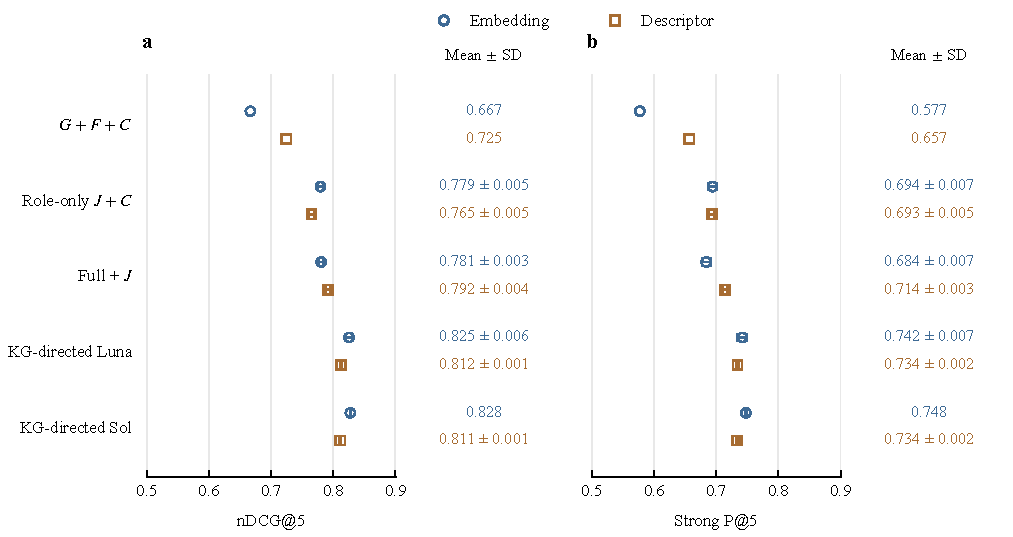
\includegraphics[width=\textwidth]{figure2_observer_comparison.pdf}
\caption{Observer comparison on the common gallery and query panel: a, nDCG@5; b, Strong P@5. Circles and squares identify the embedding and descriptor representations. Points report three-collection means; capped error bars show sample SD across collection means. Numerical SDs below 0.001 are omitted for clarity; all error bars retain their actual values. The fixed $G+F+C$ control is deterministic. $J$ is holistic Luna support: Full+$J$ retains the initial score, whereas $J+C$ ranks the inherited eligible pool by visual support alone. KG-directed Luna and Sol use clause coverage $H$.}
\label{fig:performance}
\end{figure*}



Relative to $G+F+C$, KG-directed Luna increases mean nDCG@5 by 0.1586 and 0.0878. Holistic visual assessment also improves the initial ranker: Full+$J$ reaches $0.7806\pm0.0034$ and $0.7915\pm0.0036$. The additional mean advantages from clause-directed acquisition are therefore 0.0447 and 0.0210. Their Holm-adjusted $p$ values are 0.0908 and 0.0508; neither meets the planned 0.05 threshold. Sol-minus-Luna changes are +0.0022 and -0.0012, with adjusted $p=1$ for both. The positive mean differences are consistent with a benefit from requirement-directed observation, although uncertainty across roles prevents a confirmed advantage after multiplicity correction. Complete comparisons and intervals appear in Supplementary Section~S3.

\subsection{Contribution of the scoring components}

Table~\ref{tab:paired} presents a stagewise component ablation. The screened
$G+C$ ranker provides the geometric anchor. Removing one component from Full
gives $A+F+C$, $G+A+C$, $G+F+C$ and $G+A+F$, exposing the respective contributions
of geometry, function support, exemplar-category agreement and size eligibility.
The final two rows then compare
holistic and clause-directed visual evidence on the same Full score.

\begin{table*}[t]
\centering\small
\begin{tabular}{@{}lrrrr@{}}
\toprule
Scoring configuration & \multicolumn{2}{c}{Embedding} & \multicolumn{2}{c}{Descriptor} \\
\cmidrule(lr){2-3}\cmidrule(lr){4-5}
 & nDCG@5 & Strong P@5 & nDCG@5 & Strong P@5 \\
\midrule
$G+C$ & $0.528$ & $0.475$ & $0.266$ & $0.228$ \\
$A+F+C$ & $0.649$ & $0.597$ & $0.649$ & $0.597$ \\
$G+A+C$ & $0.523$ & $0.460$ & $0.556$ & $0.502$ \\
$G+F+C$ & $0.667$ & $0.577$ & $0.725$ & $0.657$ \\
$G+A+F$ & $0.328$ & $0.285$ & $0.428$ & $0.389$ \\
Full: $G+A+F+C$ & $0.628$ & $0.546$ & $0.714$ & $0.642$ \\
\midrule
Full+$J$ (role-only) & $0.781\!\pm\!0.003$ & $0.684\!\pm\!0.007$ & $0.792\!\pm\!0.004$ & $0.714\!\pm\!0.003$ \\
Full+$H$ (KG, Luna) & $0.825\!\pm\!0.006$ & $0.742\!\pm\!0.007$ & $0.812\!\pm\!0.001$ & $0.734\!\pm\!0.002$ \\
\bottomrule
\end{tabular}

\caption{Stagewise component ablation on the same 264 queries. LLM entries are mean $\pm$ sample SD over three response collections. Deterministic rows give fixed-checkpoint scores without an SD; execution-order repeats do not measure training-seed variability. $G,A,F$ denote geometry, exemplar-category agreement and category-derived role support; $C$ is measured-size screening. Active score components have equal weights. $J$ is holistic role-only Luna support; $H$ is KG-directed Luna coverage. Formal comparisons appear in the supplement.}
\label{tab:paired}
\end{table*}



Measured screening increases Full nDCG@5 over its unscreened score by 0.3004 and 0.2860. Removing geometry changes Full by +0.0213 for embeddings and -0.0644 for descriptors. The $G+F+C$ control exceeds Full by 0.0387 and 0.0108, showing that exemplar-category agreement can reduce the initial score's effectiveness. Component contributions therefore depend on the representation and on conflicts between geometric and category-derived evidence. Visual assessment supplies an additional, role-specific signal rather than assuming that every initial component is beneficial.

\subsection{Role-dependent evidence effects}

Figure~\ref{fig:families} resolves the difference from holistic assessment by role.

\begin{figure*}[t]
\centering
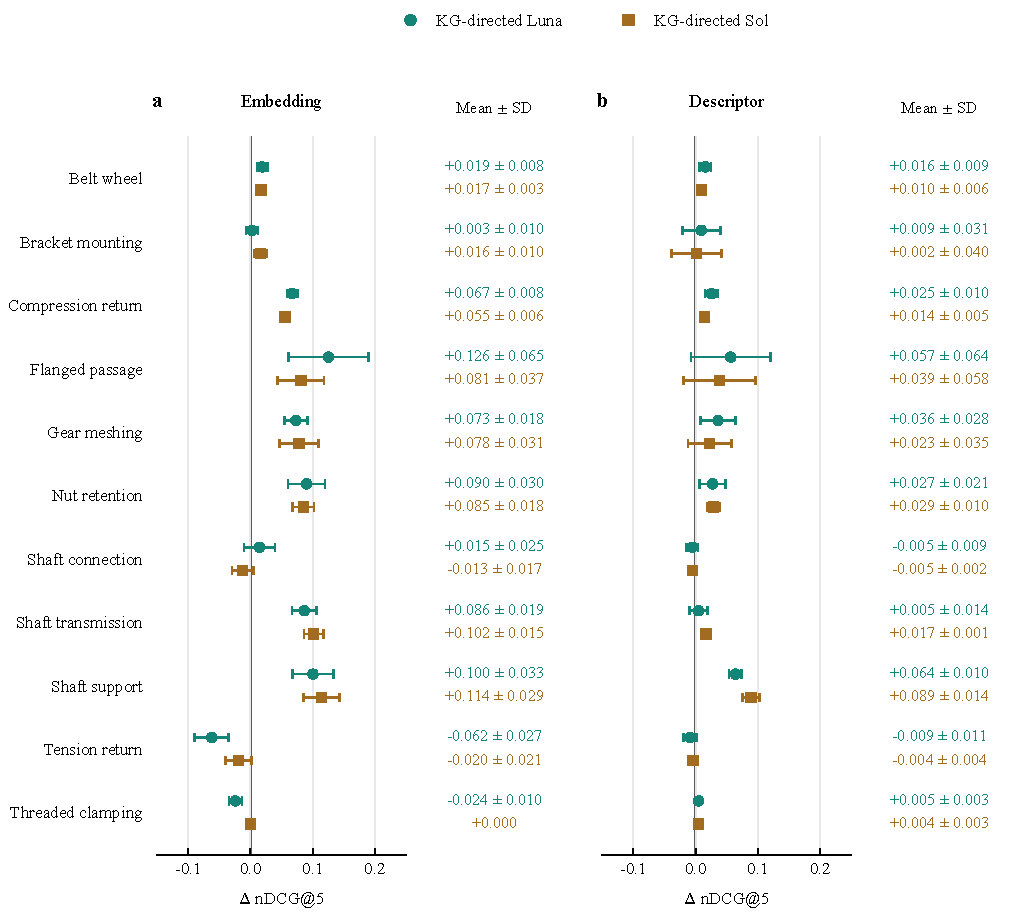
\includegraphics[width=\textwidth]{figure3_role_differences.pdf}
\caption{Role-specific nDCG@5 differences from the Full+$J$ holistic Luna control: a, embedding; b, descriptor. Numerical labels show mean $\pm$ sample SD of three paired collection differences. SD labels below 0.001 are omitted; error bars retain their actual values. Each collection averages four exemplars and six size conditions within the role. Positive values favour KG-directed observation; the vertical reference marks zero. Luna compares observation designs with the same model. Sol also changes the observer and is descriptive. These SDs describe acquisition variation, not confidence intervals across roles.}
\label{fig:families}
\end{figure*}

KG-directed Luna improves the mean in nine roles and reduces it in two for each representation. The largest embedding gains occur for flanged passage (0.1255) and shaft support (0.1004); these roles also lead the descriptor gains, at 0.0566 and 0.0640. Their requirements distinguish a passage from a visible recess and a mountable carrier from a generally annular form. In Luna collection 1, annular candidate Z1527 receives holistic support $J=0.75$ but coverage $H=0.375$: the seat is observed, mounting and carrier form are rejected, and their binding is unknown. The holistic description also notes uncertain mounting. Clause aggregation makes that missing required structure explicit in the ranking signal.


Compression and tension return share the spring-category prior, yet their effects differ. Compression gains are 0.0670 and 0.0254; tension changes are -0.0622 and -0.0086. For paired-coil candidate Z0939, the AI reference accepts opposed tensile attachments. KG-directed Luna gives $H=0.25$ in collections 2 and 3, assigning no to both hook clauses and the required opposite-end binding on one coil; holistic Luna gives $J=0.875$. This case combines visual interpretation differences with a restrictive single-coil requirement. Relationship scope therefore matters to functional coverage. The observations and qualitative selection procedure are supplied in Supplementary Section~S4.

\subsection{Source-linked explanation of a ranking change}

Figure~\ref{fig:evidence} links observations from the retained first Luna collection to a descriptor shaft query. Exemplar Q0054 is an elongated stepped shaft with integral drive features. Its classifier assigns spring probability 0.9706 and shaft probability 0.0067. Base \Full{} consequently ranks bearing Z0430 first through strong agreement with the incorrect exemplar prediction. The graph-directed observations assign no to all four shaft clauses for this short annular body and yes to all four for splined shaft Z0972, giving $H=0$ and $H=1$.

\begin{figure*}[t]
\centering
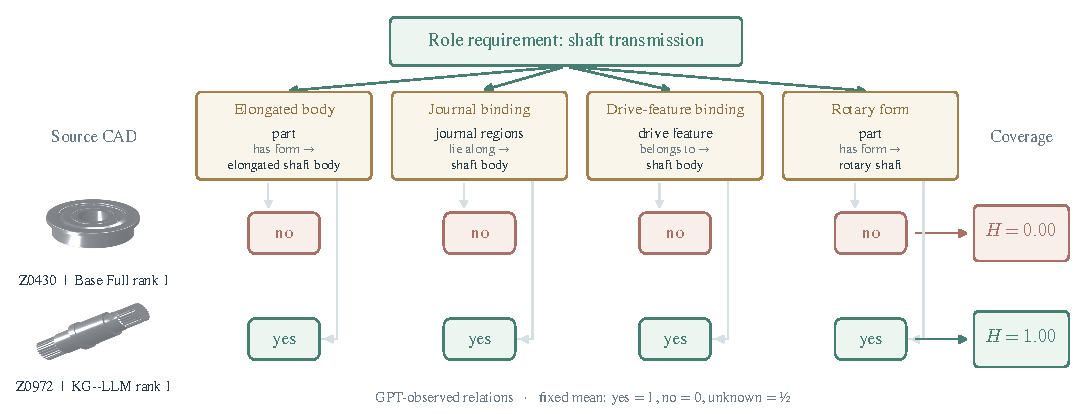
\includegraphics[width=\textwidth]{llm_evidence_graph.pdf}
\caption{Source-linked KG evidence for descriptor shaft retrieval with exemplar Q0054 and extent bound 235.25~mm. The role specifies four geometric clauses and their component bindings. Observations from Luna collection 1 give Z0430 coverage 0 and Z0972 coverage 1. That collection moves Z0972 from Base Full rank 4 to rank 1; Z0430 has reference grade 0 and Z0972 grade 2. Both pass the serving dimensional screen. Metallic rendering reuses source-bound CAD surfaces with independent display scales; materials are illustrative. View citations and complete observation descriptions accompany each graph record. The case illustrates a ranking mechanism selected after aggregate analysis.}
\label{fig:evidence}
\end{figure*}



Refinement promotes Z0972 from fourth to first and increases this query's nDCG@5 from 0.2773 to 0.8688, matching $G+F+C$. The visible shaft interfaces counteract the misleading category agreement while retaining the original score terms. The explanation identifies the precise evidence that changes the order. Coverage remains an observation-based signal: another high-coverage candidate in the same shortlist, Z0821, has reference grade 0 under the elongated-journal role scope. The model describes a splined articulated assembly, whereas the reference rejects its short coupling form. This disagreement identifies role scope and geometric interpretation as priorities for expert assessment. Supplementary Section~S4 examines an additional case involving dimensional-reference uncertainty.

\subsection{Interpretation and limitations}

The controls locate the contribution at the level of evidence acquisition.
Full and the role-only hybrid share the same geometric and category-derived score;
the proposed module changes how visible support is requested and aggregated.
The graph organizes the requirements, their bindings and observation provenance.
An information-matched flat implementation can reproduce the same initial algebra.
The comparison tests the requirement-guided acquisition and aggregation procedure.

Repeated collection assesses stochastic observer variability conditional on a
single validation-selected encoder and an unchanged query design. Three collections provide a limited estimate of acquisition variation. The AI-derived reference has no
independent expert adjudication and may share visual assumptions with the tested
observers. Historical inspection, descriptor-conditioned exemplar selection and
related CAD designs constrain generalization. Materials, loads, tolerances and
mating compatibility require subsequent engineering assessment. The bounded
refinement pool also limits recovery to candidates reached by the initial branches.


\section{Conclusions}

A knowledge-guided relational-evidence method connects requested CAD functions
to authored geometric predicates, view-linked model observations and deterministic
coverage. Measured dimensions govern candidate eligibility. Three collections per
observer evaluate acquisition variability on 1,816 CADs and 264 queries across
eleven roles. KG-directed Luna reaches nDCG@5 of 0.8254 and 0.8125, with corresponding Sol values of 0.8275 and 0.8112. Luna exceeds the matched holistic control by 0.0447 and 0.0210 in mean nDCG, with positive effects in nine roles per representation; the corrected tests remain inconclusive. Component ablation separates geometric and category-derived
signals, dimensional screening and visual acquisition. The resulting evidence is
traceable to source views and supports preliminary functional discovery within
the evaluated AI-graded collection.

\section*{Data and code availability}
Accompanying materials provide numerical results, figure-generation scripts,
role requirements, observation contracts, source-linked model assessments and
ranking records. Retained responses support metric reconstruction without
additional model calls; complete replay uses the original source dataset.
TMCAD is available through its original source \cite{zou2025brt}.

\section*{Declaration of AI-assisted manuscript preparation}
OpenAI Codex assisted with manuscript organization, reference checking,
visualization code and figure development. OpenAI image generation supplied a
layout concept for Figure~\ref{fig:framework}, which was reconstructed with
editable graphics and source CAD renders. The authors retain responsibility
for final verification, editing and approval of the article.

\par\vspace{6pt}
{\fontsize{7.5}{8.7}\selectfont
\interlinepenalty=10000
\input{references.bbl}
}
\end{document}
